%==================================================================================================
%   LUKES THESIS TEMPLATE 1.2
%   -------------------------
%   This template is based upon the offcial IMM PhD Thesis template, it is enhanced with a number
%   of new features and a number of errors have fixed. This template is intended to be complied to
%   PDF using PDFLATEX and is tested using the MiKTeX 2.9 LaTeX distribution.
%   It is based on the official DTU-IMM Thesis template by Finn Kuno Christensen in 2009.
%   Small bugfixes by Kasper Laursen in 2012 and 2013.
%   Small updates by Finn Kuno Christensen/Henning Christiansen in 2015.
%   -------------------------
%   Last Updated: 2015-01-08
%==================================================================================================
%
%==================================================================================================
% DOCUMENT SETUP
%==================================================================================================
\documentclass[10pt,twoside]{book}                  %Official DTU-IMM Thesis document setup
%
%Set to 'print' for printed version, use 'net' for online version
\def\thesisversion{net}
%
%==================================================================================================
% PACKAGES
%==================================================================================================
\usepackage{LukeThesis}                             %Import Thesis base style
%input{PhDMacros}                                   %Thesis specific macros
%
%==================================================================================================
% THESIS PROPERTIES (Modifiy these fields with your details)
%==================================================================================================
\def\thesisauthor{Alessandro Dal Corso}                     %Author
\def\thesistitle{Hybrid techniques for photorealistic rendering}               %Title
\def\thesishandin{01-April}                       %Submission date (Day-Month}
\def\thesisdegree{PhD}                              %Degree ('B.Eng', 'B.Sc.', 'M.Sc.' or 'PhD')
\def\thesisyear{2017}                               %Submission year
\def\thesisnumber{????}                             %DTU-IMM Serial number (do not include year)
\def\thesisISSN{0000-0000}                          %ISSN number
\def\thesiskeywords{rendering, materials}  %PDF keywords
\derivethesisprops                                  %Derive dependent properties
%
%==================================================================================================
% SECTION NUMBERING SETUP
%==================================================================================================
\setcounter{tocdepth}{2}                            %2 adds sections up to subsections
\setcounter{secnumdepth}{3}                         %Subsubsections get a number when this is 3
%
%==================================================================================================
% THESIS STRUCTURE  (Modifiy to include more chapters etc)
%==================================================================================================
\begin{document}
%------------------------
%Pre-frontmatter material
%------------------------
\prefrontmatter
%--------------------
%Frontmatter material
%--------------------
\frontmatter
\pagenumbering{roman}                               %Set frontmatter numbering style
\chapter{Summary}

Interactive rendering applications are becoming more and more prominent in every day life. In many fields in manufacturing, product design and entertainment, photorealistic rendering is becoming more and more prominent, in order to correctly predict the appearance of complicated materials. However, in many interactive applications, there is a need for fast interactive techniques that achieve physically based results. 

In this thesis, we address the challenge of proposing new photorealistic interactive rendering techniques, that leverage the parallel power of graphics processing unit (GPUs) in order to effectively create renderings that are physically based. These techniques exploit caching and filtering schemes in order to efficiently reuse data, both spatially and temporally.     
 
This thesis offers insight into different areas of computer graphics, including scene reconstruction, material parameter estimation, efficient data structures and physically based rendering models. In addition, we explore the different compromises and trade-offs that are necessary to achieve accurate photorealistic renderings. More specifically, we contribute with two innovative technique, one related to fast rendering of translucent materials, including directional effects of subsurface scattering into consideration. Our other technique contributes with a fast reprojection scheme to improve temporal stability in interactive ray tracing, that can be easily applied on top of existing algorithms. On top of these, we propose an innovative validation pipeline to compare renderings with actual images, with the final purpose of validating existing rendering and reconstruction techniques. 

With these contributions, this thesis proves how it is possible to use effective caching schemes to effectively improve existing techniques to handle more complex optical effects, maintaining the time constraints of interactive rendering environments.                                   %English summary of Thesis
\markboth{}{}                                       %Set headings (left)(right)
\chapter{Summary (Danish)}
\begin{otherlanguage}{danish}

\end{otherlanguage}                                   %Danish summary of Thesis
\markboth{}{}                                       %Set headings (left)(right)
\chapter{Preface}

The work from this Ph.D. thesis was carried under the Section for Image Analysis and Computer Graphics, at the Department for Applied Mathematics and Computer Science (DTU Compute) at the Technical University of Denmark (DTU). This thesis was prepared in fullfillment of the requirements to obtain a doctor of philosophy (Ph.D.) in computer science. The work presented was funded on a DTU Compute internal scholarship. 

This thesis deals with the topic of bringing techniques from photorealistic offline rendering into the interactive and real time domain. To achieve this goal, a set of publications was produced over the course of the studies. These publications that are summarized at page~\pageref{sec:contributionlist}. The publications are available in Appendices~\ref{sec:firstcontribution}-\ref{sec:robdataset}. From these, a total of five peer reviewed publications have been included in this thesis (\ref{sec:firstcontribution}-\ref{sec:lastcontribution}), while two (\ref{sec:virtualtable}-\ref{sec:robdataset}) have been left out as not relevant to the overall thesis topic. Moreover, during the course of the Ph.D. some notes were produced. These notes are grouped as non peer reviewed material and attached in Appendices~\ref{sec:jensennote}-\ref{sec:mertensnote}. 

The work has been carried under the main supervision of Associate Professor Jeppe Eliot Revall Frisvad, with the co-supervision of Associate Professor Andreas B\ae rentzen. The research activies have mostly been conducted at DTU, with the exception of two external research stay periods. The first research stay was an internship at NVIDIA Corporation, under managers Aaron Lefohn and David Luebke, in the real time rendering research team based in Redmond, Washington, USA. The second external research stay was under the supervision of Professor Toshiya Hachisuka, Department of Creative Informatics, The University of Tokyo.

%==================================================================================================
% SIGNATURE AREA
%==================================================================================================
\vspace{20mm}
\begin{center}
    \hspace{20mm} Lyngby, \thesishandin-\thesisyear
    \vspace{5mm}
    \newline
  %Update signature image file in line below
    
\includegraphics[scale=0.5]{figures/signature}
\end{center}
\begin{flushright}
    \thesisauthor
\end{flushright}
% % % EOF % % %                                     %Preface
\markboth{}{}                                       %Set headings (left)(right)
\chapter{Acknowledgements}

First and foremost, I would like to thank my supervisors Jeppe Revall Frisvad and Andreas B\ae rentzen. In particular, I would like to thank Jeppe for the support during the PhD, the deep technical discussions and a push to strive for perfection. I would like to thank Andreas for the deep and interesting discussion on how to push my work towards more and more challenging directions. I would also like to thank my managers and mentors during my internship at the real-time rendering research group in NVIDIA: Craig Kolb, Marco Salvi, Aaron Lefohn and David Luebke, for sharing some of their deep knowledge about graphics. Finally, I would like to thank Toshiya Hachisuka and its group for hosting me at Tokyo University, for the their hospitality and the interesting discussions.

I would like to thank DTU Compute for financing my scholarship and giving me the opportunity to pursue a PhD in the realm of computer graphics.

A great thank you of course goes to my colleagues, collaborators, and office mates at the section for Image Analysis and Computer Graphics. Thank you for the continuous support, the coffee calls, and the general silliness that makes everyday a fun day to come to the office. It has been a great pleasure to be part of this section, sharing thoughts and ideas, and having interesting discussion over a coffee.

Last but not least, I would like to thank my loving family and friends. Without your continuous support and help, I would not have been able to complete this endeavor.                             %Acknowledgements
\markboth{}{}                                       %Set headings (left)(right)
%------------------
% Table of contents
%------------------
\newpage\mbox{}\newpage
\chaptermark{Contents}
\pdfbookmark{\contentsname}{toc}
\renewcommand{\sectionmark}[1]{\markright{#1}}
\sectionmark{Contents}
\addtolength{\parskip}{-\baselineskip}
\tableofcontents
\addtolength{\parskip}{\baselineskip}
\renewcommand{\sectionmark}[1]{\markright{\thesection\ #1}}
%-------------
% Main content
%-------------
\mainmatter
%\include{Chapter1}                                  %Chapter 1
%\include{Chapter2}                                 %Chapter 2
\appendix
\chapter{Scene reassembly after multimodal digitization and pipeline evaluation using photorealistic rendering}
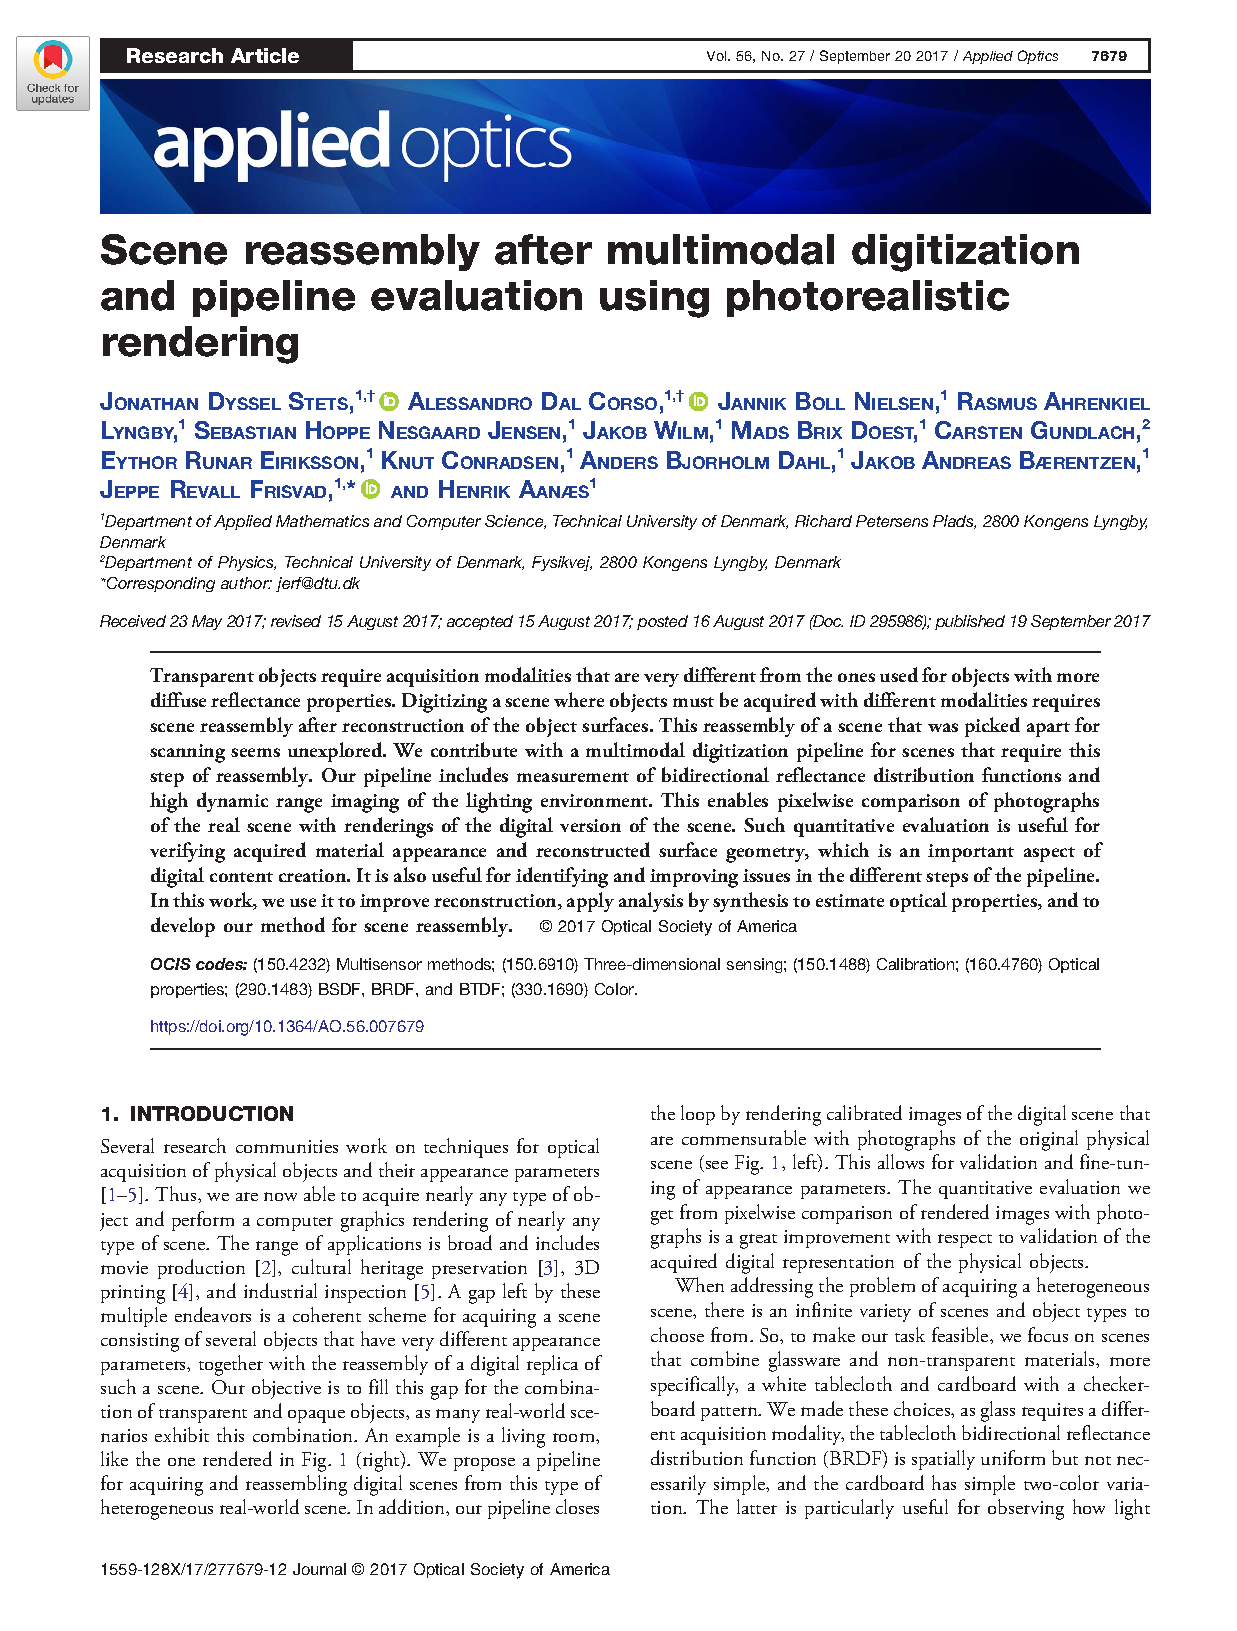
\includepdf[pages={-}]{papers/ao-56-27-7679.pdf}

\chapter{Interactive Appearance Prediction for Cloudy Beverages}
\includepdf[pages={-}]{papers/juice_mam16_submitted.pdf}

\chapter{Interactive Directional Subsurface Scattering and Transport of Emergent Light}
\includepdf[pages={-}]{papers/dirsssgpu_visual_computing.pdf}

\chapter{Interactive Stable Ray Tracing}
\includepdf[pages={-}]{papers/stable_rt_final.pdf}

\chapter{Virtual Reality inspection and painting with measured BRDFs}
\includepdf[pages={-}]{papers/abstract.pdf}

\chapter{Note on measuring BSSRDFs}
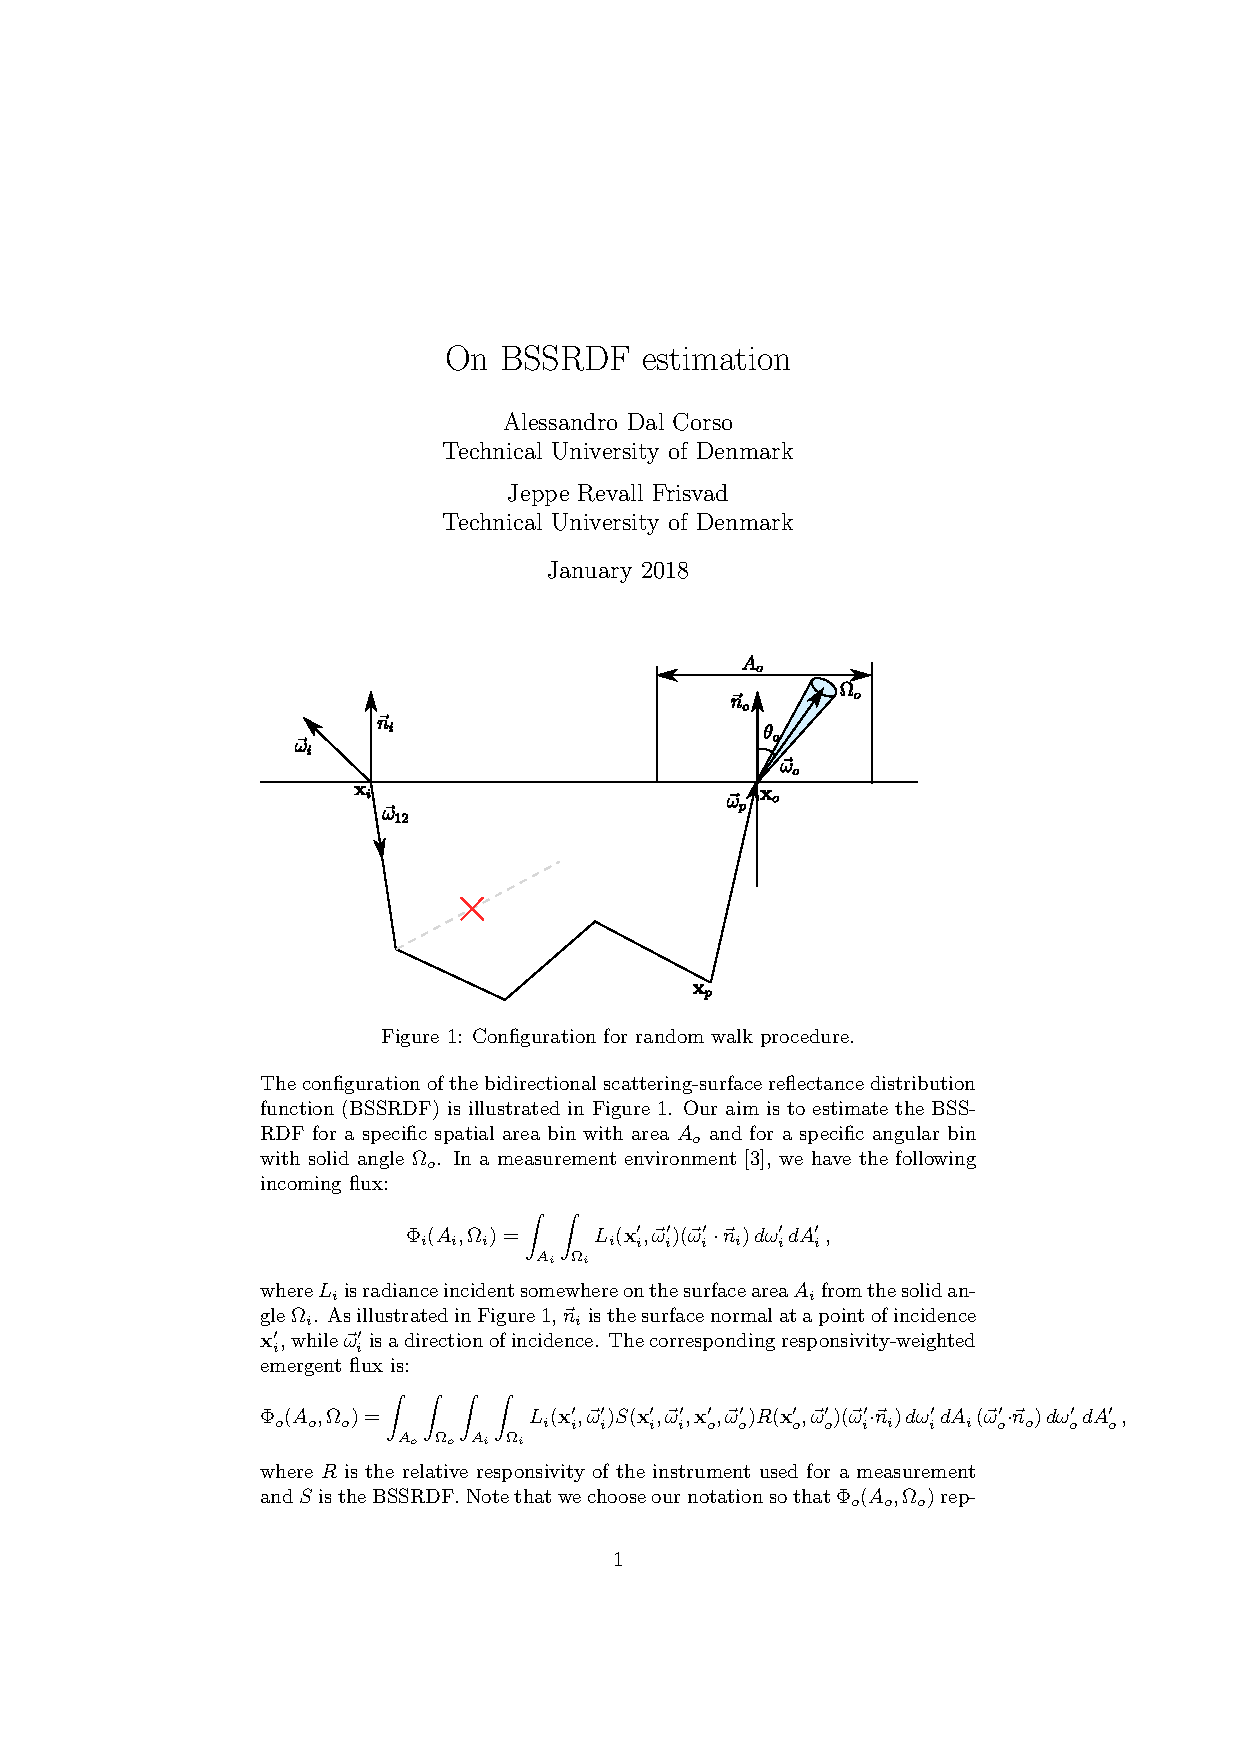
\includepdf[pages={-}]{papers/bssrdf_note.pdf}

\chapter{Note on efficient color calibration on the GLASS project}
\includepdf[pages={-}]{papers/color_calibration_note.pdf}

\chapter{Note clarifying BSSRDF importance sampling by Mertens et al.}
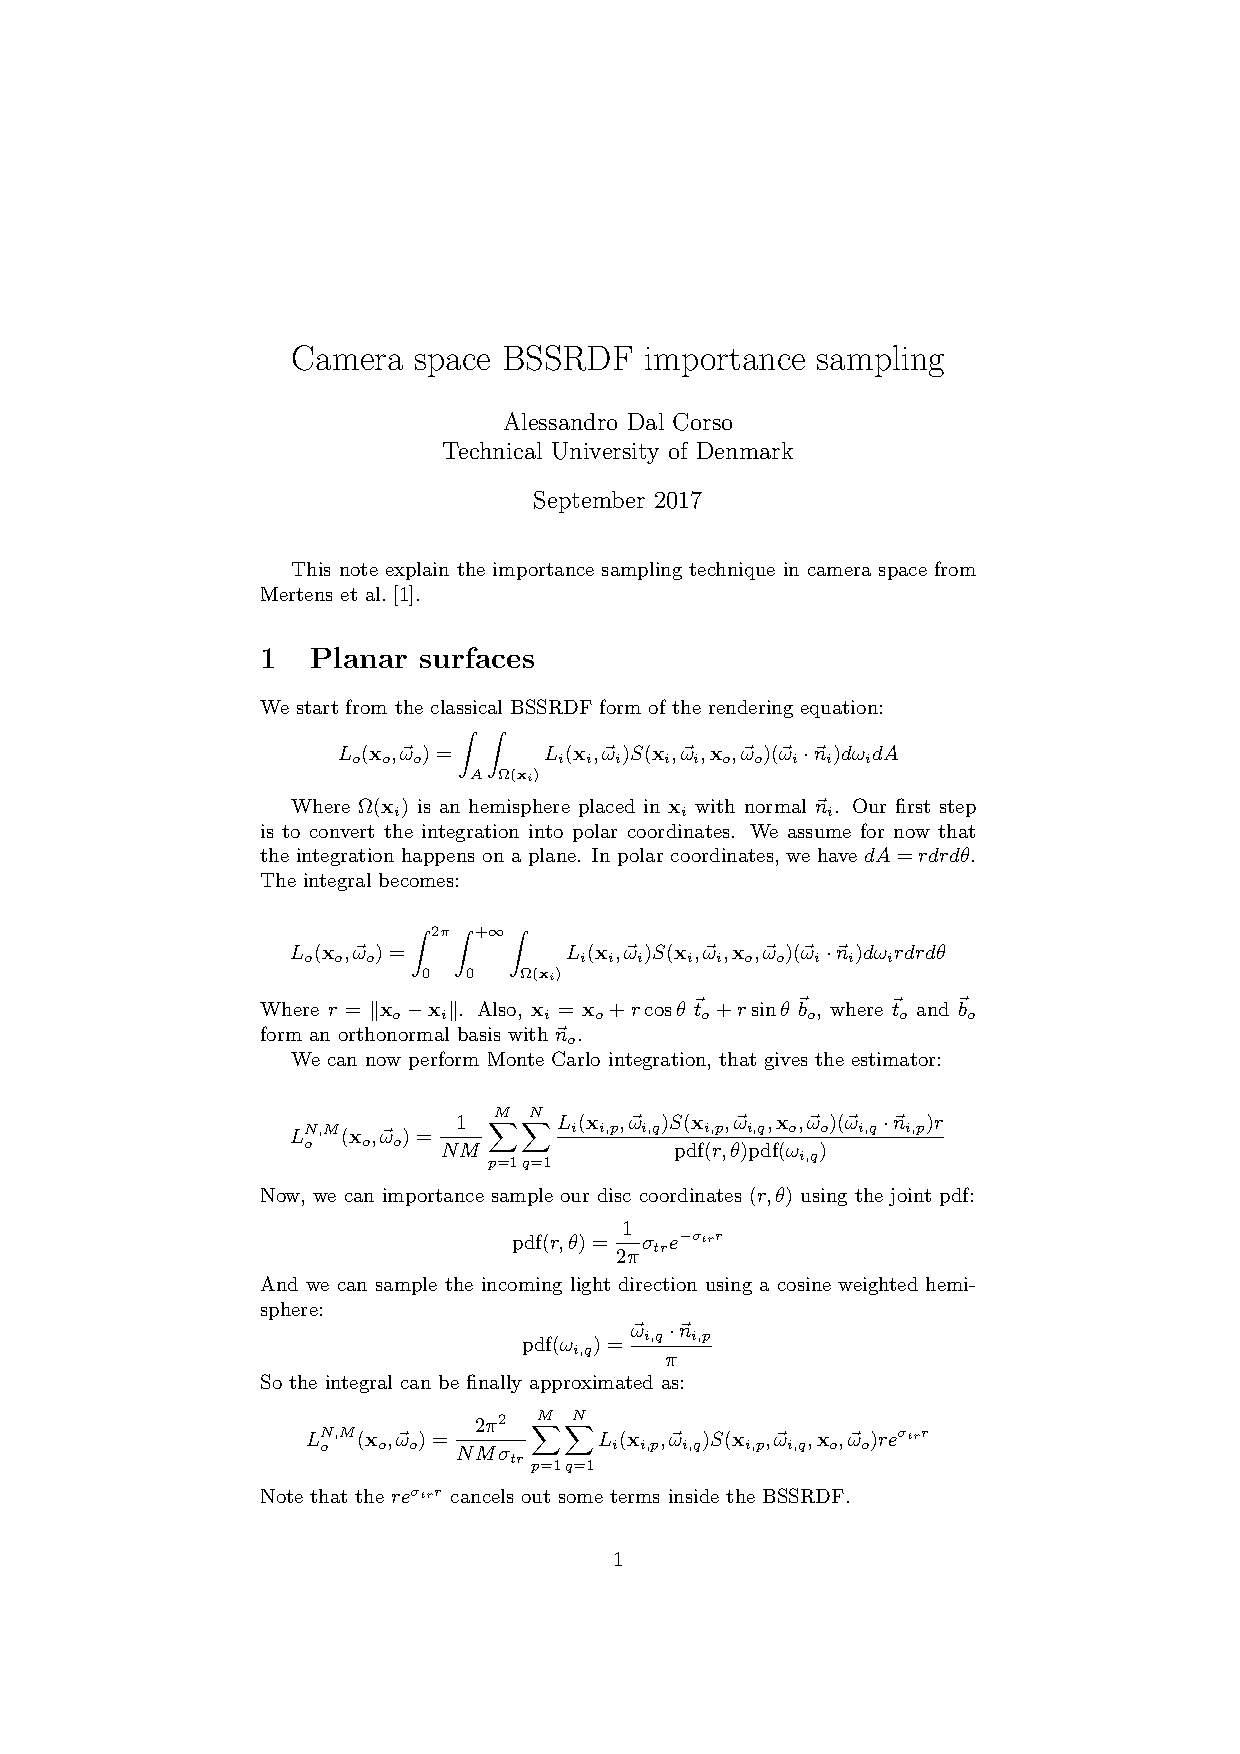
\includepdf[pages={-}]{papers/mertens_note.pdf}

\chapter{VirtualTable: a projection augmented reality game}
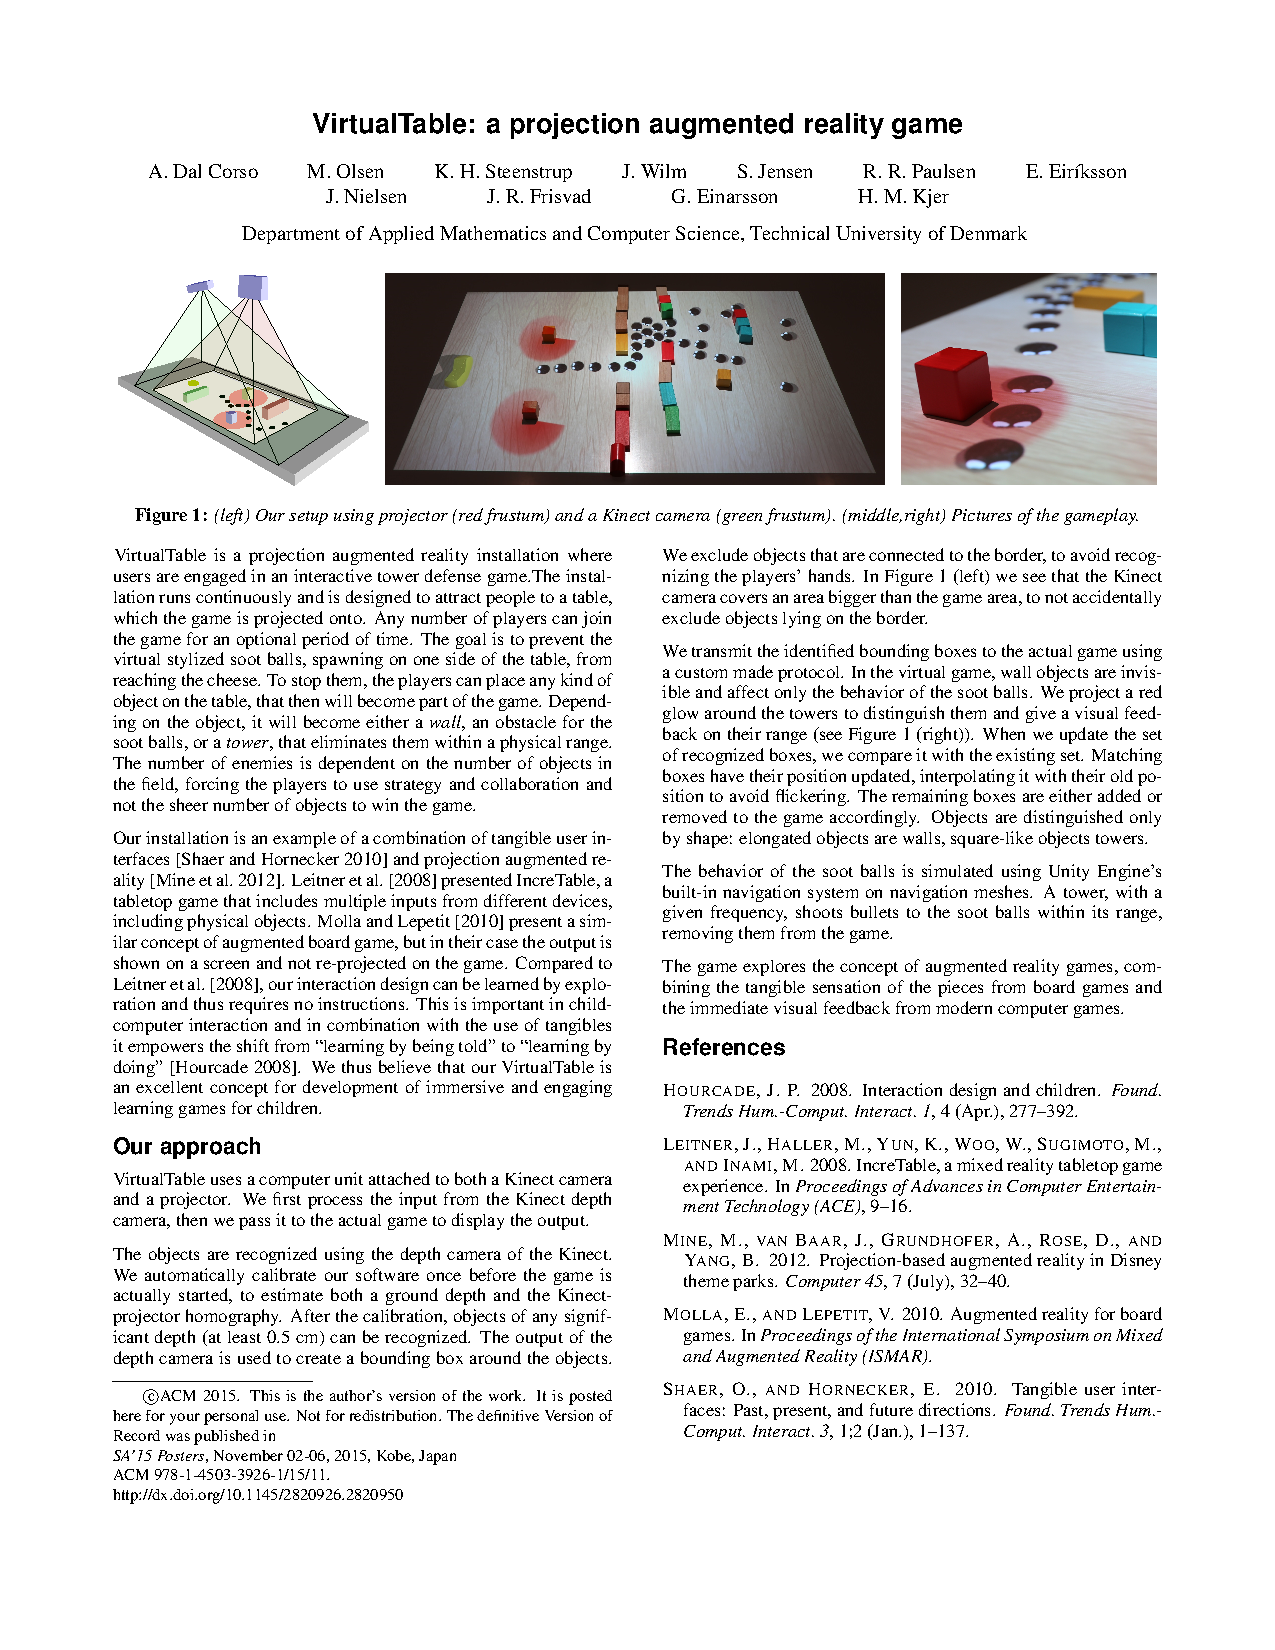
\includepdf[pages={-}]{papers/poster_siggraph.pdf}

\chapter{Our 3D Vision Data-Sets in the Making}
\includepdf[pages={2-}]{papers/robds.pdf}

                                 %Appendix A
%-----------
% Backmatter
%-----------
\backmatter
\chaptermark{Bibliography}
\renewcommand{\sectionmark}[1]{\markright{#1}}
\sectionmark{Bibliography}
\addcontentsline{toc}{chapter}{Bibliography}        %Force addition of Bibliography to TOC
\bibliographystyle{alpha}                           %Use alpha codes for references
\bibliography{references}                           %Bibliography file called
\end{document}
% % % EOF % % %